\section{Combine algebraic geometry with abstraction techniques}
\subsection{History of abstraction on sequential circuits}
Traditional method to analyze a sequential circuit is based on explicit state variable encoding
and full states enumerating from initial state and explicit transition function.
With the size of modern sequential circuits increasing, it is infeasible to apply old methods
any longer. Abstraction is a technique to minimize the state space by combining states with certain 
similarities. Sometimes it can effectively lower down the number of states by orders of magnitude,
without affecting the properties we need to verify.

At first abstraction is done manually by designers. In 2000 E. Clarke \cite{clarke2000counterexample}
proposed an automated abstraction: first,
initial abstraction is set up by dividing variables to different clusters based on transition conditions;
then, an ordinary model checking is operated on this abstraction. If a counterexample is given, 
it is further checked to be concrete or not. For a false abstract state or a spurious path 
, the initial abstraction is refined by further splitting the false abstract state. 
A heuristic algorithm keeps refining the abstraction until a real counterexample is found or 
property verified. This technique is based on binary decision diagrams (BDDs), which means
potential risk of memory explosion; meanwhile it still requires an initial abstraction to start with.
So in 2004 L. Zhang and M. Hsiao \cite{zhang2005design} proposed another abstraction method based on CNF-SAT.
This paper uses simplest latch abstraction -- by removing "irrelevant" latches and change them to primary inputs. 
The key idea is to pick those ``irrelevant" latches (variables in $k$-bounded model checking, $k$-BMC) 
according to SAT/UNSAT analysis from $k$-BMC. It improves the $k$-BMC procedure\cite{biere1999symbolic}: 
LTL properties to check for a $k$-bounded machine can be translated to a big CNF and fed to SAT solver. 
If SAT, a concrete counterexample is found. 
If UNSAT, the original method will just increase bound k. In Zhang's paper, the clauses for UNSAT 
(UNSAT cores) are checked for variables do not appear, they are referring to "irrelevant" latches 
at least for first $k$ iterations. 
Thus an abstracted model is obtained and checked with original property. If the abstracted model checking fails, 
then bound $k$ will increase. This method still has disadvantages: it is counterexample-independent,
which means it cannot utilize information from invariants.

Abstraction usually means over-approximation, i.e. properties are true on abstracted machine
are also valid for original states. Craig's interpolation is a sort of abstraction which could be both
over-approximation and under-approximation. In 2003 K. McMillan used Craig's interpolation to improve 
$k$-BMC \cite{mcmillan2003interpolation}. Initially a $k$-length path to failure state $F$ is picked and transformed to 
CNF formula, then split at first transition into prefix and suffix. Then an interpolation $P$ is computed
between prefix and suffix. $P$ over-approximates 1-step reachable states, and under-approximates states 
that cannot reach $F$ in $k$ steps. If no counterexample exposed, path will be split again at second
transition; in this way a precise abstraction can be found for all reachable states.

$k$-BMC with interpolation is a purely incremental model checking approach, and interpolation procedure relies
on UNSAT core analysis. To overcome these weaknesses, a hybrid model checker named as IC3 is developed 
\cite{bradley2011sat} \cite{bradley2011incremental}. (Not related to abstraction really..)
\subsection{Word-level abstraction: Naive abstraction for arithmetic circuits}
Our approach is an abstraction based on word operand definition of datapaths in arithmetic circuits,
and it can be expanded to generic FSM by bundling a set of bit-level variables to one or several word-level variables.
The abstraction polynomial is obtained through computing GB of an elimination ideal using a special term order.

The authors of \cite{pruss:dac14} showed that for any combinational
logic block, a canonical word-level polynomial representation can be
derived through \Grobner bases computed with elimination
orders. Our approach is based on their result, which we reproduce
here:
\begin{Lemma}
(From \cite{pruss:dac14}) Given a combinational circuit $C$ with $k$-bit
  input $A = (a_0, \dots, a_{k-1})$ and $k$-bit output $R = (r_0, \dots,
  r_{k-1})$. Denote by $x_1, \dots, x_d$ all the bit-level
  variables of   $C$. Let $J = \langle f_1, \dots, f_s \rangle \subset
  \Fkk[x_1, \dots, x_d, R, A]$ denote all the polynomials corresponding to the
  logic gates of the circuit. Let $J_0 = \langle x_1^2 - x_1, \dots,
  x_d^2 - x_d, R^q - R, A^q - A \rangle$ be the vanishing ideal, so
  that $J + J_0 = \langle f_1, \dots, f_s, ~~ x_1^2 - x_1, \dots,
  x_d^2 - x_d, R^q - R, A^q - A \rangle$. Compute \Grobner basis $G =
  GB(J + J_0)$ w.r.t. lex term order with $x_1 > x_2 > \dots > x_d > R
  > A$. Then $G_d = G \cap \Fkk[R, A]$ eliminates the internal
  variables $x_1, \dots, x_d$ of the circuit. $G_d$ also contains the
  word-level polynomial $R = \F(A)$ which canonically represents the
  function of the circuit.  
\end{Lemma}

The authors referred to the elimination (lex) order with
$\{\textit{internal variables} \ x_1 > \dots > x_d\} > \{\textit{word-level
  output} \ R\} > \{\textit{word-level input} \ A\}$ as the {\it abstraction
  term order (ATO)}. 
  
One-step transition can also be implemented on word level using ATO. We represent present state (PS) 
with a univariate polynomial about word-level state variable $f(S)$, its variety intersecting with variety of
circuit ideal $J+J_0$ results to polynomial about word-level next state (NS) $g(T)$. Recall theorem \ref{thm:unionintersect},
$$NS = {\bf V}(\langle g\rangle) = {\bf V}(\langle f\rangle + J+J_0) = GB\ with\ ATO(\langle f\rangle + J+J_0)$$
Note that ideal corresponding to next state is an ideal with single univariate polynomial generator.

Reachability analysis is a useful tool when checking sequential equivalence as well as other invariants.
With word-level state variables, we can do implicit state enumeration to provide a picture of 
reachable states. Following algorithm is breadth-first search style state enumeration \cite{KallaPartialScan}:
\begin{algorithm}[hbt]
\SetAlgoNoLine
 \KwIn{Transition functions $\Delta$, initial state $S^0$}

  $from^0 = reached = S^0$\;
  \Repeat{$new^i == 0$}
  {
  	$i \gets i + 1$\;
	$to^i \gets$Img$(\Delta, from^{i-1})$\;
	$new^i \gets to^i \cap \overline{reached}$\;
  	$reached \gets reached \cup new^i$\;
	$from^i \gets new^i$\;
  }
\Return{$reached$}
\caption {Breadth-first Traversal Algorithm}\label{alg:BFS}
\end{algorithm}
\begin{figure}[hbt]
\centering{
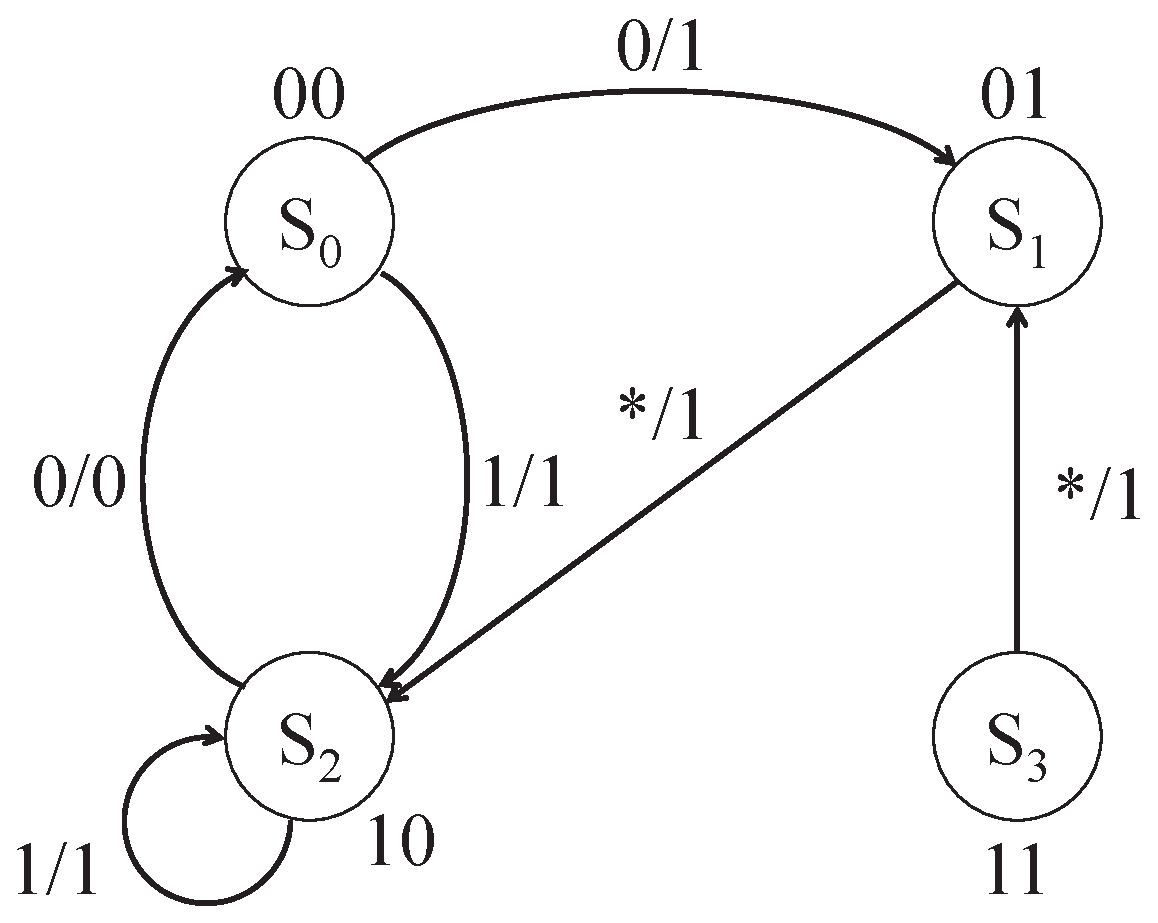
\includegraphics[scale=0.3]{./stg_fig.eps}
\caption{State transition graph of sample FSM}
\label{fig:stg}}
\end{figure}

\begin{figure}[hbt]
\centering{
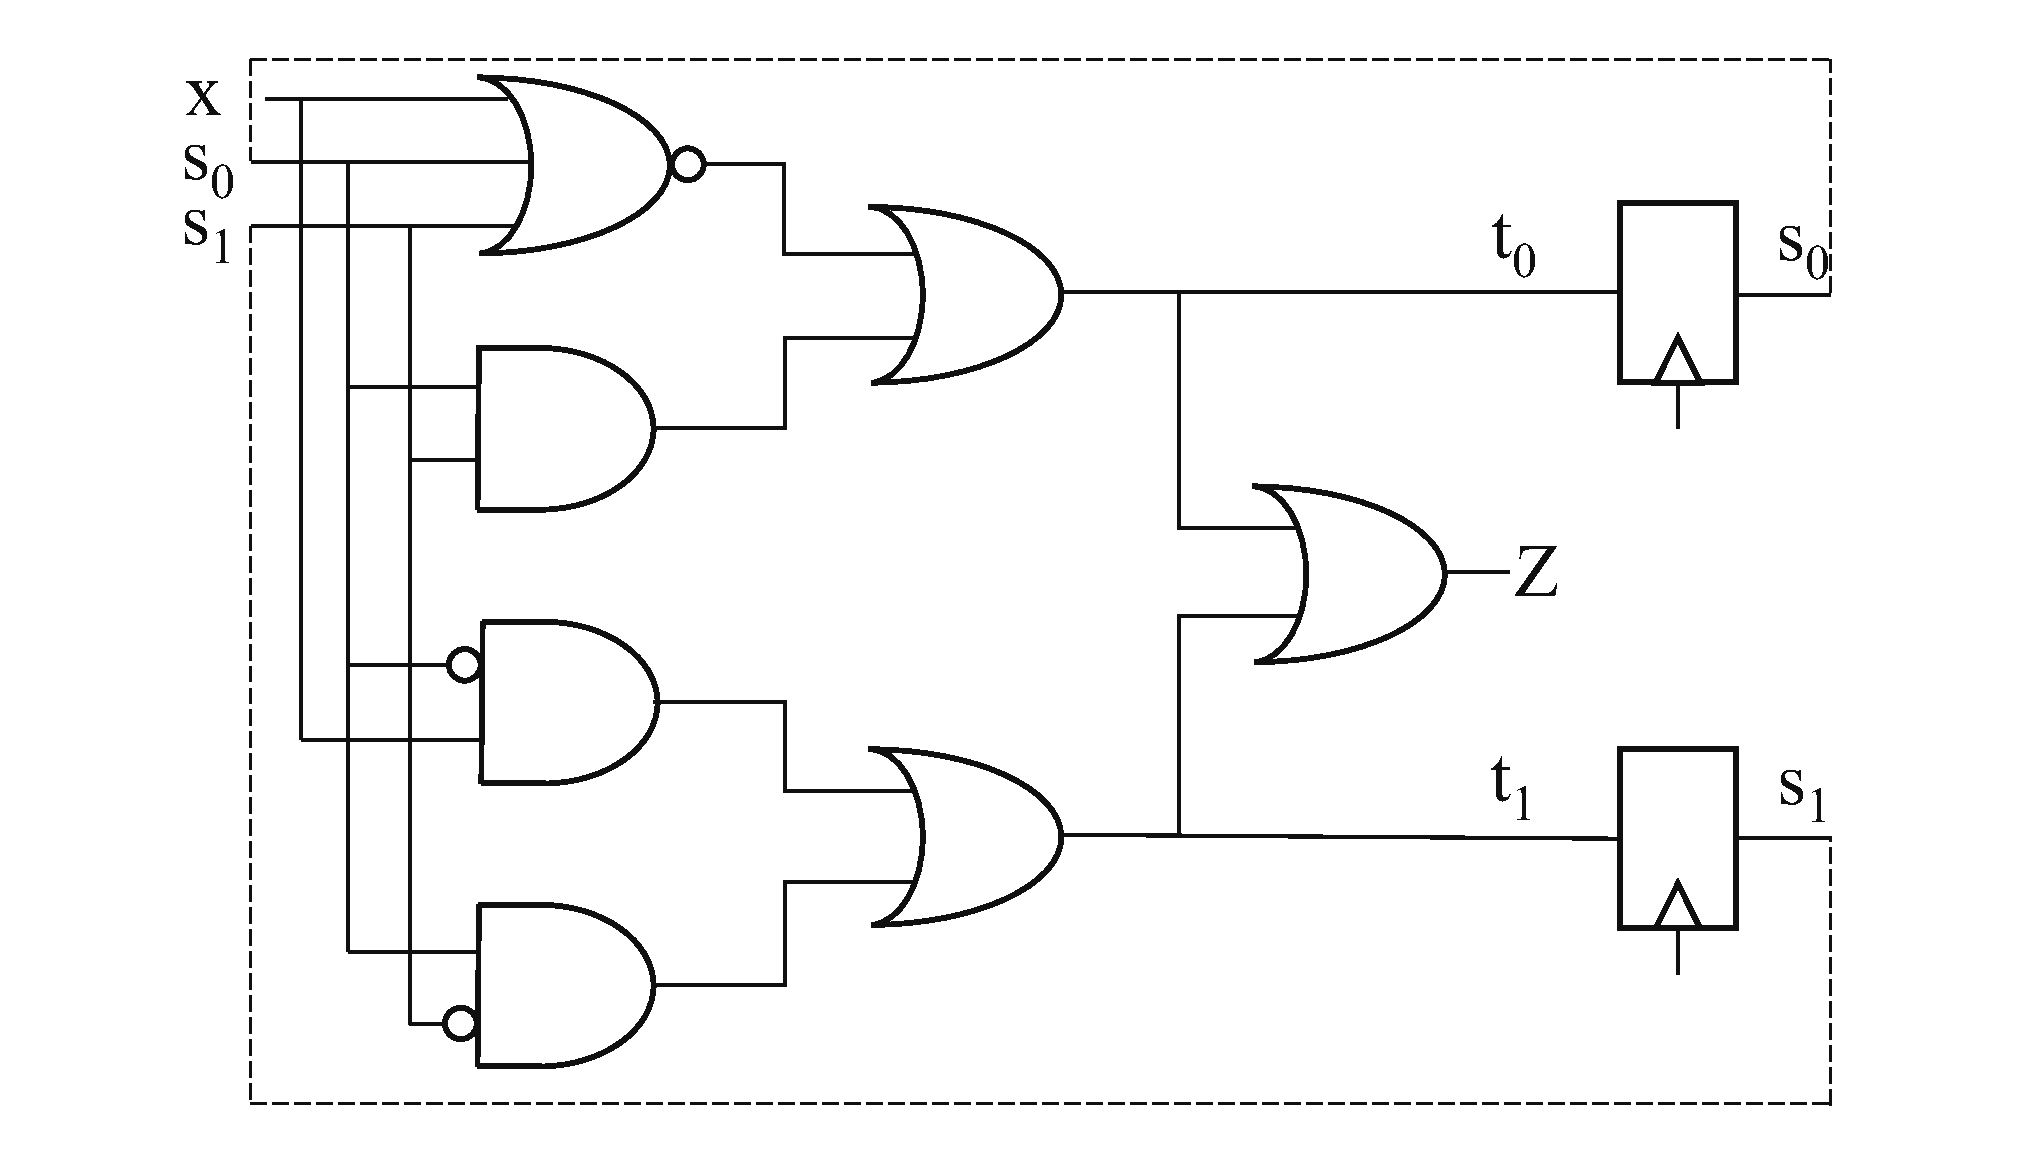
\includegraphics[width=3.5in]{./fsm_fig.eps}
\caption{Gate-level circuit of combinational logic block of sample FSM}
\label{fig:fsm}}
\end{figure}
Here we put a 2-bit Mealy machine as an example showing how to use univariate polynomial ideal
and elimination ideal with ATO to implement this algorithm.
\begin{Example}
\label{ex:2bit}

We are given a mealy Finite State Machine (FSM). Gate-level circuits of combinational logic
is figure \ref{fig:fsm}, $x$ is primary input (one bit),
$\{s_0, s_1\}$ are state inputs, $Z$ is primary output and $\{t_0, t_1\}$ are state outputs.
Word-level state input is $S = s_0 + s_1\cdot\alpha$, output is $T = t_0 + t_1\cdot\alpha$. In Galois field
$\mathbb{F}_{2^2}$, bit-level variables $x, s_0, s_1, Z, t_0, t_1$ can take values from $\{0, 1\}$, while
word-level variables $S, T$ may take values from $\{0, 1, \alpha, 1 + \alpha\}$. State Transition Graph (STG)
showed in figure \ref{fig:stg} uses 2-bit Boolean vector to represent 4 states $\{S_0, S_1, S_2, S_3\}$, which
could be mapped to elements in $\mathbb{F}_{2^2}$.

For example in Line 1 of BFS algorithm, assume initial state is $S_0$ in figure \ref{fig:stg}, then corresponding
polynomial $f = \mathcal{F}(S^0) = S^0 - 0$. Consider an ideal $I$ with only one generator $f$, its variety
$V(I) = \{\gamma\ |\ \gamma \in \mathbb{F}_{2^2}, \gamma = 0\}$, which equals to $\{0\}$, the only
valid value $S^0$ can take.

If an ideal contains multiple polynomial specifications, it is necessary to compute Gr\"obner basis with elimination term
order to get one polynomial only on desired variable. In first iteration of Line 4, $to^i$ has multiple specifications,
some of them are transition functions on bit-level:
\begin{displaymath}
\begin{array}{ll}
f_1:& t_0 - (\overline{x}\ \land\ \overline{s_0}\ \land\ \overline{s_1})\ \lor\ (s_0\ \land\ s_1) \\
f_2:& t_1 - (\overline{s_0}\ \land\ x)\ \lor\ (s_0\ \land\ \overline{s_1})\
\end{array}
\end{displaymath}
And some are bits-to-word definitions using polynomial representation of elements in $\mathbb{F}_{2^2}$:
\begin{displaymath}
\begin{array}{ll}
f_3:& S - s_0 - s_1\alpha \\
f_4:& T - t_0 - t_1\alpha
\end{array}
\end{displaymath}
And an polynomial about initial state as mentioned above:
\begin{displaymath}
f_5:\  S
\end{displaymath}
And the rests are vanishing polynomials for every variable, bit-level and word level:
$f_6: x^2 - x; f_7: t_0^2 - t_0; f_8: t_1^2 - t_1; f_9: S^4 - S; f_{10}: s_0^2 - s_0;
f_{11}: s_1^2 - s_1; f_{12}: T^4 - T$

Note that there is no specification on initial primary input $x$, in Gr\"obner basis approach this means $x$ is smoothed by
reversely using Shannon's expansion.

Employing elimination term order: $intermediate\ bit$-$level\ signals\ >\ bit$-$level\ primary\ inputs/outputs\ >\ S\ >\ T$, compute Gr\"obner basis for ideal
$J = \langle f_1, f_2, \dots, f_{12}\rangle $, the result will include one polynomial $f_T$ contains only variable $T$. In this example,
$f_T = T^2+(\alpha+1)T+\alpha$. This polynomial equals to $T^2-(\alpha+1)T+\alpha$ since coefficients of polynomial representation in $\mathbb{F}_{2^2}$ are
limited within $\mathbb{F}_{2}$, where $x \equiv -x\ (mod\ 2)$ for any element $x$ in the field. Solution to $f_T = 0$ is $T = 1\ or \ T = \alpha$, which shows that next
state the machine just reached is $\{S_1(01), S_2(10)\}$.

Continue to run this traversal algorithm, it will terminates with final reachable states $f_T = T^3+(\alpha+1)T^2+\alpha T$, its solution is $T=0\ or\ T=1\ or\ T=\alpha$,
which shows within total 4 states, state $S_3$ is unreachable from initial state $S_0$.

When executing Line 5 and Line 6, use \textbf{union}, \textbf{intersection} and \textbf{complement} of varieties over $\mathbb{F}_{2^k}$. Since
state set variables $from^i, to^i, reached$ all have single polynomial generator, consider an ideal $I$ with single generator $I = \langle f\rangle $.
For example, assume $I = \langle f\rangle  = \langle T^2 + (1+\alpha)\cdot T+\alpha\rangle $, its variety $V(I) = \{a\ |\ a \in \mathbb{F}_{2^2}\ and\ f(a) = 0\} = \{1, \alpha\}$.

For varieties intersection $\{1\}\bigcap\{1, \alpha\}$, calculate ideal sum $\langle T+1, T^2 + (1+\alpha)\cdot T+\alpha\rangle  = \langle T+1\rangle $,
its variety is $\{1\}$; for varieties union $\{1,\alpha\}\bigcup\{1+\alpha\}$, calculate
ideal product $\langle (T+1+\alpha)\cdot(T^2 + (1+\alpha)\cdot T+\alpha)\rangle  = \langle T^3 + 1\rangle $, its variety
is $\{1, \alpha, 1+\alpha\}$; for complement set of variety $\{1, \alpha\}$, the universal set is
the variety of ideal of vanishing polynomial $V(\langle T^4-T\rangle ) = \{0,1,\alpha,1+\alpha\}$,
so $\overline{V(\langle T^2 + (1+\alpha)\cdot T+\alpha\rangle )} = V(\langle T^4-T\rangle ) - V(\langle T^2 + (1+\alpha)\cdot T+\alpha\rangle )$,
which equals to $V(\langle T^4-T\rangle :\langle T^2 + (1+\alpha)\cdot T+\alpha\rangle ) = V(\langle T^2+(1+\alpha)\cdot T\rangle )$,
the result is $\{0,1+\alpha\}$.

From discussion above, the BFS traversal is completely implemented in Galois field.
If the initial input is $S_3$: $S + 1 + \alpha$, the final return value will be set of
reachable states: $T^4 + T$, i.e. the universal set, $\{S_0, S_1, S_2, S_3\}$. Modified algorithm could be
written in following interpretation:

\begin{algorithm}[hbt]
\SetAlgoNoLine
 \KwIn{Input-output circuit characteristic polynomial ideal $I_{ckt}$, initial state polynomial $\F(S)$}

  $from^0 = reached = \F(S)$\;
  \Repeat{$new^i == 1$}
  {
  	$i \gets i + 1$\;
	$to^i \gets$GB w/ elimination term order$\langle I_{ckt}, from^{i-1}\rangle$\;
	$new^i \gets $generator of $\langle to^i\rangle + (\langle T^4-T\rangle:\langle reached\rangle)$\;
  	$reached \gets $generator of $\langle reached\rangle \cdot \langle new^i\rangle$\;
	$from^i \gets new^i(S\setminus T)$\;
  }
\Return{$reached$}
\caption {Algebraic Geometry based Traversal Algorithm}\label{alg:univa}
\end{algorithm}

Here $from^i, to^i, new^i$ are all univariate polynomials about $S$ or $T$.
\end{Example}

\subsection{Obviate GB computation}
% Introduce: RATO
% Get word-level output -- bit-level inputs function
% Use bit variable substitution to finish word-level abstraction
Elimination ideal with ATO technique requires a GB computation, which is usually infeasible on large designs.
To obviate GB computation, we introduce a refinement on ATO as well as bit-word substitution method.

To overcome high computational complexity of GB calculation, \cite{pruss:dac14} proposed a
\underline{r}efinement of ATO (called RATO), and simplified the
\Grobner basis computation. They exploited Buchberger's product
criteria \cite{productc:1979}, which states that: {\it If the leading  
monomials of $f_i, f_j$ are relatively prime, then $Spoly(f_i, f_j)$
reduces to zero modulo the generating set, i.e. $Spoly(f_i, f_j)
\xrightarrow{F} _+ 0$.} This concept was exploited in RATO as follows: 

Perform a reverse topological sorting of the nodes in the
combinational logic, and define a {\it lex} term order by the
following relation $>_{r}$: {\it bit-level circuit variables ordered
  reverse topologically} $>$  {\it word-level output variables} $>$
{\it word-level input   variables}. Representing the polynomial ideal
$J$ in RATO has the effect that there exists {\it one and only one
  pair of polynomials} in $J$ that do not have relatively prime
leading terms (see  Section 5 in \cite{pruss:dac14} for details). All
other polynomial pairs will have leading terms that are 
relatively prime, so these polynomial pairs are not considered in
Buchberger's algorithm.  The authors of \cite{pruss:dac14} exploited
this concept and showed how the \Grobner basis of $(J + J_0)$ can be
computed by a {\it subset} of polynomials, which  improves the
scalability of their approach. Their approach, however, cannot
circumvent the \Grobner basis computation altogether. Consequently, 
their approach fails to derive a canonical polynomial abstraction when
the representation is dense, and contains monomials of high-degrees
(e.g. in case of buggy designs). 

It turns out that RATO can be applied to sequential circuits in much
the same way: {\it \{bit-level circuit variables ordered
  reverse topologically} $x_1 > \dots x_d\}$ $>$  {\it \{word-level NS
  variables} $R'> A'> B'\}$ $>$ {\it \{word-level PS variables}
$R>A>B\}$. Importantly, {\it we show that using RATO, the polynomial
abstraction can be derived without resorting to a \Grobner basis
computation.} Perform the following operations: 

\begin{enumerate}
\item Represent the polynomials of the sequential circuit $S$ using RATO.
\item Due to RATO, only one pair of polynomials ($f_i, f_j$) will have
  leading terms that will not be relatively prime.
\item Reduce $Spoly(f_i, f_j) \xrightarrow{F}_+ h$.
\end{enumerate}
As described in \cite{pruss:dac14}, remainder $h$ will contain:
  i) the word-level variables, and ii) bit-level inputs to the
  combinational logic, i.e. bit-level present-state variables. All
  other internal circuit variables will not appear in $h$, as they
  will be canceled by division due to RATO. 

However with only RATO, the final remainder $h$ contains both bit-level variables and
word-level {\it state variables}. We desire
a polynomial in only word 
level variables without computing a
\Grobner basis. This can be achieved if we  represent the
bit-level state variables in terms of their word-level
variables. We exploit 
the following property of finite fields:

\begin{Lemma}
\label{lemma:square}
For $\alpha_1, \dots, \alpha_t \in \Fkk$, $(\alpha_1 + \alpha_2 +
\dots + \alpha_t)^{2^i} = \alpha_1^{2^i} + \alpha_2^{2^i} + \dots +
\alpha_t^{2^i}$, for $i = 1, 2, \ldots$. 
\end{Lemma}

Consider the polynomials that define the relationship between the
word-level and bit-level variables. Let 
$ A = a_0 \beta + a_1\beta^2 + \dots + a_{k-1}\beta^{2^{k-1}}$.
Due to Lemma \ref{lemma:square}, we have $A^2 = a_0 \beta^{2}+ a_1
\beta^{4} + \dots + a_{k-1} \beta^{2\cdot 2^{k-1}}$ (as
$a_i^2 = a_i$). By repeated squaring:
\begin{eqnarray}
A & = & a_0 \beta + a_1\beta^2 + \dots + a_{k-1}\beta^{2^{k-1}}\nonumber\\
A^2 & = & a_0 \beta^{2}+ a_1 \beta^{4} + \dots + a_{k-1}
\beta^{2\cdot 2^{k-1}} \nonumber\\
\vdots & \vdots& \vdots \nonumber\\
A^{2^{k-1}} & = & a_0 \beta^{2^{k-1}}  +  a_1 \beta^{2^{k-1}\cdot 2} +
\dots + a_{k-1}\beta^{2^{2(k-1)}} \nonumber
\end{eqnarray}
% \alert{Some concern that we do not show that this system of equations is always
% uniquely solvable.}
Consider the above as $k$ {\it linear equations} with $a_0, \dots, a_{k-1}$
as $k$-unknowns, with $\beta$ and its powers as coefficients, and 
$A, A^2, ... \dots, A^{2^{k-1}}$ as $k$ constants. Then, we can solve
for the unknowns $a_0, \dots, a_{k-1}$ and obtain expressions for them
in terms of $A$ and $\beta$. The problem can be setup in
matrix form:

\begin{displaymath}
\begin{pmatrix}
\beta & \beta^2 & \cdots & \beta^{2^{k-1}} \\
\beta^2 & \beta^4 & \cdots & \beta^{2^{k-1}\cdot 2} \\
\vdots & \vdots & \ddots & \vdots \\
\beta^{2^{k-1}} & \beta^{2^{k-1}\cdot 2} & \cdots & \beta^{2^{2(k-1)}}
\end{pmatrix}
\begin{pmatrix}
a_0\\
a_1\\
\vdots\\
a_{k-1}
\end{pmatrix}
=
\begin{pmatrix}
A\\
A^2\\
\vdots\\
A^{2^{k-1}}
\end{pmatrix}
\end{displaymath}

Gaussian elimination on this system of equations can be 
applied, and each bit-level variable $a_i$ can be represented as a
function of the word-level variables: $a_i = g_i(A)$. These bit-level
variables can be easily substituted in the remainder $h$ obtained by
reduction due to RATO. What we will obtain is a word-level polynomial
 which canonically represents the function of the circuit.  


Using RATO to get word-level transition function may result in multivariate polynomial generators
instead of single univariate generator. To compute NS, we intersects variety of transition ideal 
with PS (output word's function about input words, plus
evaluations of input words), then result NS may have multiple multivariate generators. 
Complement also requires multivariate ideal quotient.

\begin{Example}
Consider 2-bit FSM traversal (Ex:\ref{ex:2bit}) using RATO and multivariate polynomial generators.
Following algorithm is a modified breath-first search (BFS) traversal algorithm based on ideals with multivariate 
generators.
\begin{algorithm}[hbt]
\SetAlgoNoLine
 \KwIn{Transition polynomial $f_t = T + \mathcal F (S,x)$, 
	initial state ideal $from^0 = \langle S+\mathcal G(x), x^{q_1} - x\rangle$}

  $reached = from^0(T\setminus S)$\;
  \Repeat{$GB(new^i) == 1$}
  {
  	$i \gets i + 1$\;
	$to^i \gets$GB$(\langle f_t, from^{i-1}\rangle) \setminus \mathcal H(S)$\;
	$\overline{reached} = \langle T^{q_2}-T, x^{q_1} - x \rangle : reached$\;
	$new^i \gets $GB$(to^i + \overline{reached})$\;
  	$reached \gets $GB$( reached \cdot new^i)$\;
	$from^i \gets new^i(S\setminus T)$\;
  }
\Return{$reached$}
\caption {Algebraic Geometry based Traversal Algorithm (multivariate-generator ideals)}\label{alg:multi}
\end{algorithm}

Inputs of this algorithm are: a transition polynomial, which is the result of word-level abstraction; initial 
states description ideal, contains 2 generators defining PI could be any inputs and state inputs $S$ is a specific
value. (Ex: $\langle S+1+\alpha, x^2+x\rangle$ means initial state$=\{11\}$,
$\langle S+x\cdot\alpha, x^2+x\rangle$ means initial states$=\{00,10\}$).

Transition polynomial calculation exploits our improved RATO approach. After building
an elimination ideal, use RATO such that \emph{reverse\ topo\ order\ circuit\ variables }$> T > S > x$, the reduction
remainder has the form $T+\mathcal F(s_0,s_1,x)$. From word definition $S+s_0+s_1\alpha$ we get
$$s_0 = \alpha S^2+ (1+\alpha)S, s_1 = S^2+S$$
Do substitution, the transition polynomial of example circuit is 
$$f_T = T+S^3\cdot x+\alpha S^3+(1+\alpha)S^2\cdot x+S^2+S\cdot x+(1+\alpha)x+1$$

Assume we start from state $\{11\}$. First iteration, it will reach state $\{01\}$. Line 4 is to compose an
ideal with 2 generators from $from^0$ and transition polynomial $f_T$, compute its Gr\"obner basis. Note this ideal
has the form
\begin{equation}
I_{tran} = \left\{
             \begin{array}{c}
             T+\mathcal F(S,x) \\
             S + \mathcal G(x) \\
             v_x
             \end{array}  
        \right.
\end {equation}
$v_x$ is a polynomial containing only $x$, initially it should be vanishing polynomial $x^{q_1}-x$, with the program executing
it may be factorized.

Consider Buchberger's algorithm, all generators' leading terms are relatively prime, so it is a GB itself. 
Then we need to reduce this GB, we will find out $S + \mathcal G(x)$ could (possibly) be reduced by $v_x$,
and $T+\mathcal F(S,x)$ will definitely reduced by $S + \mathcal G(x)$. So, at last we will get a polynomial
$T + \mathcal F'(x)$ in reduce GB. We can include this polynomial and $v_x$, exclude the polynomial containing
$S$ (i.e. $\mathcal H(S)$ in algorithm), to compose an ideal representing \emph{next states} $to^i$. In iteration 1, result is $to^1 = \langle T+1, x^2+x\rangle$

Line 5 is the ideal quotient of universal set and reached states. In the first iteration, 
$reached$ is the initial state $\langle T+1+\alpha, x^2+x \rangle$. Result of ideal quotient
is $\langle T^3+(1+\alpha)T^2+\alpha T, x^2+x\rangle$ represents $\{00,01,10\}$.

Line 6 is ideals' sum (intersection of their varieties), it is done by combining all generators
from 2 ideals and compute GB. For first iteration result is $GB(\langle T+1,T^3+(1+\alpha)T^2+\alpha T, x^2+x\rangle) = \langle T+1, x^2+x\rangle$ representing $\{01\}$.

Line 7 is ideals' product (union of their varieties), it is done by multiplying all pairs of
generators from both ideal. For first iteration result is $GB(\langle (T+1)(T+1+\alpha),
(T+1)(x^2+x), (T+1+\alpha)(x^2+x), (x^4+x)\rangle) = \langle T^2+\alpha T+(1+\alpha), x^2+x\rangle$ representing $\{01,11\}$.

The traversal will run for 3 iterations and terminate at 4th iteration. We list all intermediate 
results below:
\begin{itemize}
\item Iteration 1: $from^0 = \langle S+1+\alpha, x^2+x\rangle, to^1 = \langle T+1, x^2+x\rangle,
 reached = \langle T^2+\alpha T+(1+\alpha), x^2+x\rangle$
\item Iteration 2: $from^1 = \langle S+1, x^2+x\rangle, to^2= \langle T+\alpha, x^2+x\rangle,
reached = \langle T^3+1, x^2+x\rangle$
\item Iteration 3: $from^2 = \langle S+\alpha, x^2+x\rangle, to^3 = \langle T+\alpha x, x^2+x
\rangle, reached = \langle T^3\cdot x+x, T^4+T, x^2+x\rangle$
\item Iteration 4: $from^3 = \langle S, x\rangle, to^4 = \langle T+1, x\rangle, new = \langle1\rangle$
\end{itemize}
The final reachable states are represented by ideal $\langle T^3\cdot x+x, T^4+T, x^2+x\rangle$,
which means $\{00,01,10,11\}$.
\end{Example}

\subsection{A simplified traversal on multivariate polynomial generators: SMPO}
% 1. How to design SMPO
% 2. Improved algorithm: why this can verify arithmetic function
% 3. Example of 3-bit SMPO
Sequential GF multiplier has no primary input, so it can be regarded as Moore FSM. 
The states are encoded by evaluations of state variables, which can be implicitly verified 
by checking output-input function ($R = A\cdot B \pmod P(\alpha)$). Additionally
the inner structure of GF multiplier is XOR-rich such that we can test our approach on very large
(>100 bits datapath) circuits.

Let us briefly describe the fundamentals behind the design of normal
basis sequential GF multipliers, so as to put in perspective the type
of designs that have been verified in this paper. Let $R =
\sum_{i=0}^{k-1} r_i \beta^{2^{i}}, ~A = \sum_{i=0}^{k-1} a_i
\beta^{2^{i}}, ~B = \sum_{i=0}^{k-1} b_i \beta^{2^{i}}$, then 
\[
R = A\cdot B = (\sum_{i=0}^{k-1} a_i \beta^{2^{i}}) (\sum_{j=0}^{k-1}
b_j \beta^{2^{j}})  =
\sum_{i=0}^{k-1}\sum_{j=0}^{k-1}a_ib_j\beta^{2^i}\beta^{2^j}\nonumber 
\]

The expressions $\beta^{2^i}\beta^{2^j}$ are called cross-product
terms and they can also be represented in normal basis: 
\begin{displaymath}
\beta^{2^i}\beta^{2^j} =
\sum_{n=0}^{k-1}\lambda_{ij}^{(n)}\beta^{2^n}, \ \ \lambda_{ij}^{(n)}
\in \Ftwo. 
\end{displaymath}

From the above two equations, one can see that the expression for the
$n^{th}$ digit of product $R = (r_0, \dots, r_n, \dots r_{k-1})$ is:
\[
r_n = \sum_{i=0}^{k-1}\sum_{j=0}^{k-1}\lambda_{ij}^{(n)}a_ib_j = A
\cdot M_n \cdot B^T, ~~0 \leq n \leq k-1
\]

where $M_n = (\lambda_{ij}^{(n)})$ is a binary $k \times k$ matrix over
$\Ftwo$, and it is called the $\lambda$-matrix. 
%The collection of all
%$\{M_n\}$  $\lambda$-matrices is called the multiplication
%table. 
Moreover, let $r_n = A \cdot M_n \cdot B^T$.
Then $r_{n-1} = A \cdot M_{n-1} \cdot B^T = rotate(A) \cdot M_n
\cdot rotate(B)^T$. This implies that $M_n$ is generated by right
and down cyclic shifting $M_{n-1}$. Therefore, the hardware design
of sequential GF multipliers is based on mappings of $A\cdot M_n
\cdot B^T$ into AND-XOR gates and cyclic shift operations. 

This paper verifies the implementation of two distinct 
architectures of {\it sequential multipliers with parallel output
  (SMPO)}, namely: i) the Agnew-SMPO  \cite{agnew1991implementation}
by G. B. Agnew, which is a straight-forward implementation of the
$\lambda$-matrix; and ii) the more recent, more complicated, yet very
efficient RH-SMPO \cite{RHmulti}, by Reyhani-Masoleh and Hasan,
depicted in Fig. \ref{fig:RHmulti}.  

\begin{figure}[hbt]
\centering{
%\begin{minipage}{12cm}
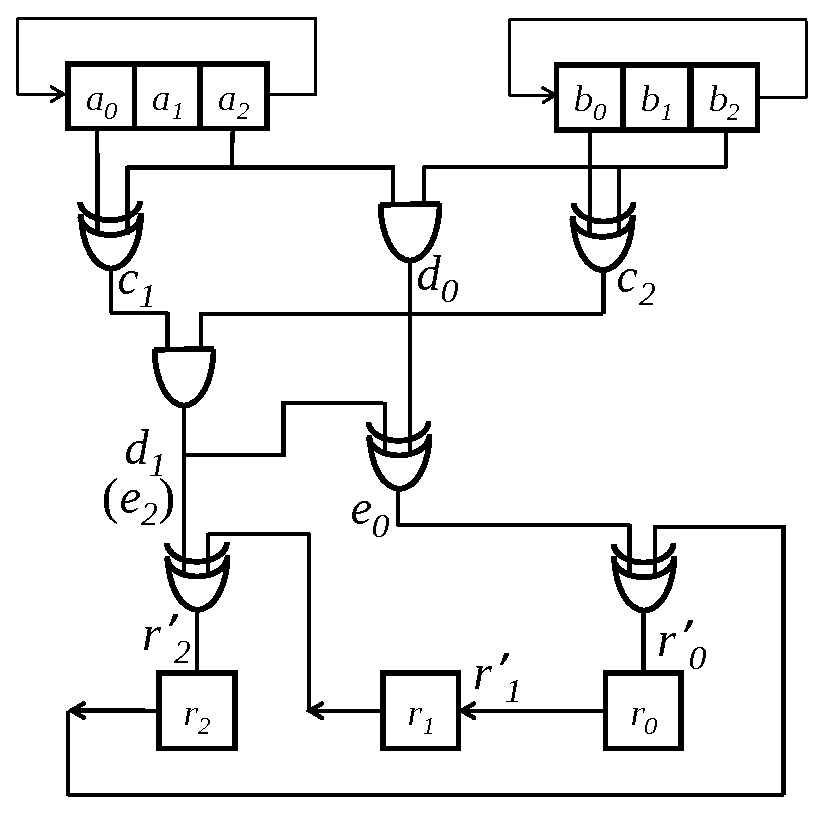
\includegraphics[width=2.25in]{./RH3.eps}
% \vspace{-0.2in}
\caption{A 3-bit RH-SMPO}
%\end{minipage}
\label{fig:RHmulti}}
\end{figure}

We follow  the typical sequential GF circuit model with word-level variables $A, B, R$
denoting {\it present states (PS)} and $A', B', R'$ denoting {\it next
  states (NS)} of the machine; where $A = \sum_{i=0}^{k-1} a_i \beta^{2^i}$
for the PS variables and $A' = \sum_{i=0}^{k-1} a_i'
\beta^{2^i}$ for NS variables, and so on.  Variables $R\ (R')$ correspond to those that 
store the result, and $A, B\ (A', B')$ store input operands. {\it E.g.,}
for a GF multiplier, $A_{init}, B_{init}$ (and $R_{init} =
0$) are the initial values (operands) loaded into the registers,  and
$R = \F(A_{init}, B_{init}) = A_{init} \times B_{init}$ is the final
result after $k$-cycles. Our approach aims to find this polynomial
representation for $R$.  

Each gate in the combinational logic is represented by a Boolean
polynomial. To 
this set of Boolean polynomials, we append the polynomials that define
the word-level to bit-level relations for PS and NS variables ($A =
\sum_{i=0}^{k-1} a_i \beta^{2^i}$). We denote this set of polynomials
as ideal $J = \langle 
f_1, \dots, f_s \rangle \subset \Fkk[x_1, \dots, x_d, R, R', A, A', B,
  B']$, where $x_1, \dots, x_d$ denote the bit-level (Boolean) variables
  of the circuit. The ideal of vanishing polynomials $J_0$ is also included, and
then the implicit FSM unrolling problem is setup for abstraction. 

The configurations of the flip-flops are the states of the
machine. {\it Since the set of states is a finite set of points, we
can consider it as the variety of an ideal related to the circuit
}. Moreover, since we are interested in
the {\it function encoded} by the state variables (over $k$-time
frames), we can {\it project this variety} on the word-level state
variables, starting from the initial state $A_{init}, B_{init}$.
Projection of varieties (geometry) corresponds to elimination ideals
(algebra), and can be analyzed via \Grobner bases. Therefore, we
employ a \Grobner basis computation with ATO: we use a {\it lex term
  order} with {\it bit-level variables} 
$>$ {\it word-level NS outputs} $>$ {\it word-level PS inputs}. This
allows to eliminate all the bit-level variables 
%(corresponding to the combinational logic and the state variables),
%so as to 
and derives a representation only in terms of words. 
Consequently, $k$-successive \Grobner basis computations implicitly
unroll the machine, and provide word-level algebraic $k$-cycle
abstraction for $R'$ as $R' = \F(A_{init}, B_{init})$. 

Algorithm
\ref{alg:modified} describes our approach.  In the algorithm, $from_i$
and $to_i$ are polynomial ideals whose varieties are the valuations of
word-level variables $R, A, B$ and $R',A',B'$ in the $i$-th iteration;
and the notation ``$\setminus$'' signifies that the $NS$ in iteration
$(i)$ becomes the $PS$ in iteration $(i+1)$. Line 5 computes the Gr\"obner 
basis with the abstraction term order.  Line 6 computes the elimination 
ideal, eliminating the bit-level variables and representing the set of 
reachable states up to iteration $i$ in terms of the elimination ideal. 
These computations are analogous to those of image computations performed in FSM reachability. 
%The forward image
%$to^{i}$ is computed using \Grobner bases with ATO.

\vspace{-0.1in}
\IncMargin{1em}
\begin{algorithm}[hbt]
\SetAlgoNoLine
\LinesNumbered
 \KwIn{Circuit polynomial ideal $J$, vanishing ideal $J_0$, initial
   state ideal $R (=0), \mathcal{G}(A_{init}), \mathcal{H}(B_{init})$} 

  $from_0(R,A,B) = \langle R, \mathcal{G}(A_{init}), \mathcal{H}(B_{init})\rangle$\;
  $i = 0$\;
  \Repeat{$i == k$}
  {
  	$i \gets i + 1$\;
%	$to^i(R',A',B') \gets$  $GB( \langle J_{ckt}, J_0,
%    from^{i-1}(R,A,B)\rangle )$ with abstraction term order\;
	$G \gets$GB$( \langle J + J_0+ from_{i-1}(R,A,B) \rangle
    )$ with ATO\;
	$to_i(R',A',B')\gets G\cap \mathbb F_{2^k}[R',A',B',R,A,B]$\;
	$from_i \gets to_i(\{R,A,B\}\setminus \{R',A',B'\})$\;
  }
\Return{$from_k(R_{final})$}
\caption {Abstraction via implicit unrolling for Sequential GF circuit
  verification}
\label{alg:modified}
\end{algorithm}
\DecMargin{1em}
\vspace{-0.1in}
\begin{Example}
\label{ex:RHSMPO}

We demonstrate our approach to verify the 3-bit RH-SMPO circuit of
Fig.\ref{fig:RHmulti}. The normal element $\beta$ in
$\mathbb{F}_{2^3}$ is known to be $\beta = \alpha^3$, where $\alpha$
is the primitive element. The circuit can be described with an ideal by translating
AND and XOR gates accordingly. For the first iteration:
\begin{align*}
J = &d_0+b_2\cdot a_2,
c_1+a_0+a_2,
c_2+b_0+b_2,
d_1+c_1\cdot c_2,\\
&e_0+d_0+d_1,
e_2+d_1,
r_0'+r_2+e_0,
r_1'+r_0,
r_2'+r_1+e_2,\\
&A+a_0\alpha^3+a_1\alpha^6+a_2\alpha^{12},
B+b_0\alpha^3+b_1\alpha^6+b_2\alpha^{12},\\
&R+r_0\alpha^3+r_1\alpha^6+r_2\alpha^{12},
R'+r_0'\alpha^3+r_1'\alpha^6+r_2'\alpha^{12};
\end{align*}
The last 4 polynomials are translated from the definition of word-level variables.
This represents ideal ``$J$" from line 5 in Algorithm
\ref{alg:modified}. ``$J_0$" is the ideal of vanishing polynomials in all bit-level
variables (e.g. $a_0^2-a_0$) and word-level variables (e.g. $A^8-A$). ``$from_{i-1}$"
% contains evaluation of PS word-level output in form of
% $R+\mathcal F(A,B)$. Since the definition of $A$ and $B$ changes after every iteration
% ($A',B'$ are different from $A, B$) and the multiplier's function only concerns about 
% initial value of $A,B$, we include the definition of $A_{init}, B_{init}$ into $from_i$:
represents the set of current states for iteration $i$.
In the first iteration, $from_0 = \{R, A_{init}+a_0\alpha^3+a_1\alpha^6+a_2\alpha^{12},
B_{init}+b_0\alpha^3+b_1\alpha^6+b_2\alpha^{12}\}$.

After the GB computation is performed with ATO, as line 6 in Algorithm \ref{alg:modified},
we find a polynomial in variables $R', A_{init}, B_{init}$ in $to_1 : 
R'+(\alpha^2) A_{init}^4 B_{init}^4+(\alpha^2+\alpha) A_{init}^4 B_{init}^2+(\alpha^2+\alpha) A_{init}^4 B_{init}+(\alpha^2+\alpha) A_{init}^2 B_{init}^4+(\alpha^2+\alpha+1) A_{init}^2 B_{init}^2+(\alpha^2) A_{init}^2 B_{init}+(\alpha^2+\alpha) A_{init} B_{init}^4+(\alpha^2) A_{init} B_{init}^2
$.

Line 7 in Algorithm \ref{alg:modified} simply replaces NS output $R'$ with PS output
$R$ in this example; so in second iteration $from_1 = \{
R'+(\alpha^2) A_{init}^4 B_{init}^4+(\alpha^2+\alpha) A_{init}^4 B_{init}^2+(\alpha^2+\alpha) A_{init}^4 B_{init}+(\alpha^2+\alpha) A_{init}^2 B_{init}^4+(\alpha^2+\alpha+1) A_{init}^2 B_{init}^2+(\alpha^2) A_{init}^2 B_{init}+(\alpha^2+\alpha) A_{init} B_{init}^4+(\alpha^2) A_{init} B_{init}^2
, A_{init}+a_2\alpha^3+a_0\alpha^6+a_1\alpha^{12},
B_{init}+b_2\alpha^3+b_0\alpha^6+b_1\alpha^{12}\}$. 

% By continue executing the loop,
Finally, after 3 iterations we obtain: $to_3 = \{ \mathbf{R'+A_{init}B_{init},}
~A_{init}+a_0'\alpha^3+a_1'\alpha^6+a_2'\alpha^{12},
~B_{init}+b_0'\alpha^3+b_1'\alpha^6+b_2'\alpha^{12}\}$
as the image. The final result is $from_3(R_{final}) = R_{final}+A_{init}\cdot
B_{init}$, which verifies the multiplier. 
\end{Example}

\subsection{Limitations: complexity of reduction (multivariate division)}
Although we gain success on verifying sequential GF multipliers, there are still problems when
doing implicit state enumerating on generic FSM. For example, when we tried to apply our approach
on ISCAS'89 benchmark s953 with 29 DFFs and 311 gates, RATO spent too much time on reducing
Spoly with ideal generators. By analyzing the process of polynomial reduction, we conjecture that
\begin{Conjecture}
Long chains of AND/OR gates will make polynomial reduction infeasible.
\end{Conjecture}

\begin{figure}[hbt]
\centering{
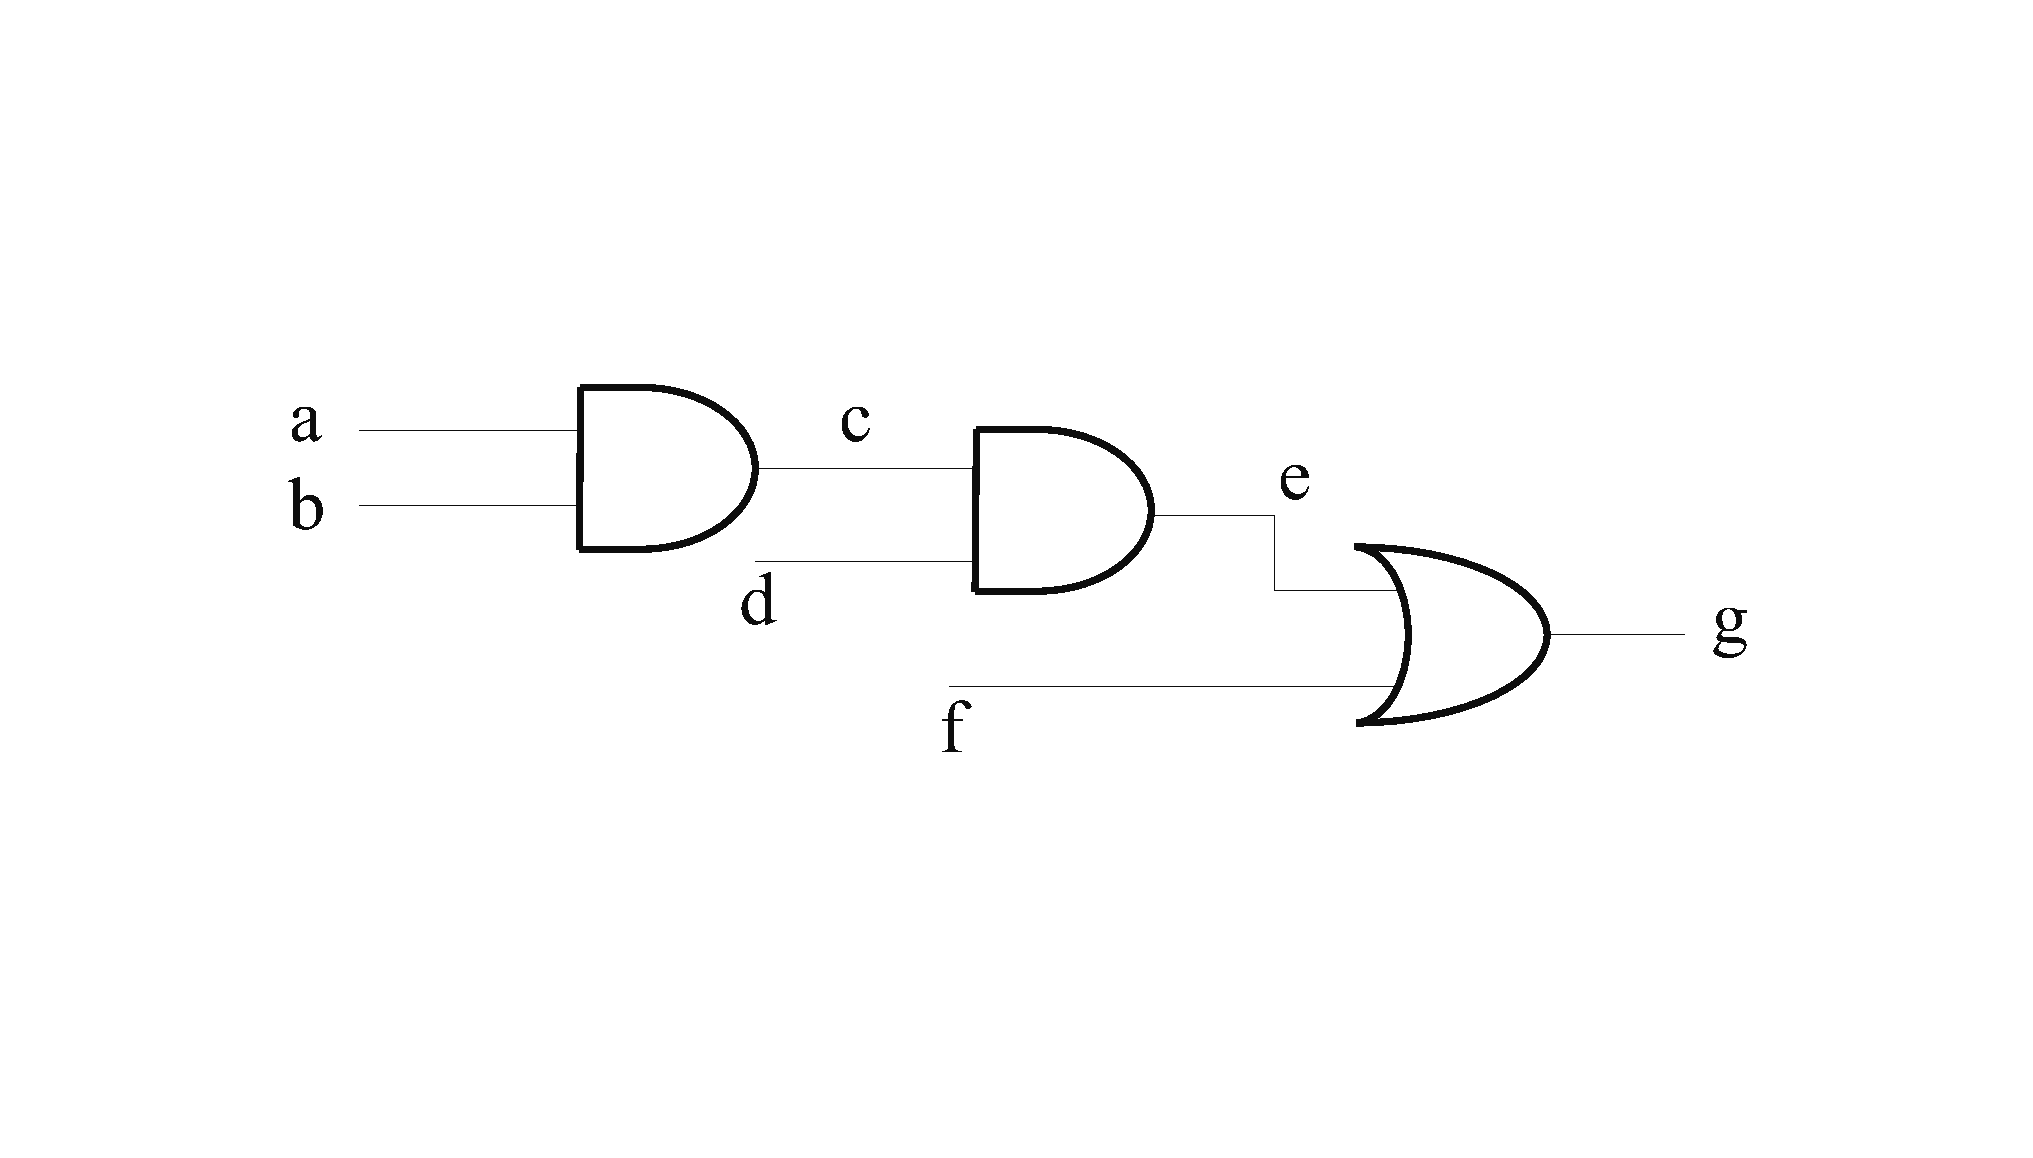
\includegraphics[scale=0.3]{./fig_chain.eps}
\caption{An example of AND-OR-gate chain}
\label{fig:chain}}
\end{figure}

\begin{Example}
Consider a chain (Fig.\ref{fig:chain}) of 3 gates: 2 AND gates and 1 OR gate. Write them in polynomials:
\begin{align*}
&h_1:g+ef+e+f\\
&h_2:e+cd\\
&h_3:c+ab
\end{align*}
Impose RATO: $g>e>c>\{a,b,d,f\}$. Reduce a simple polynomial $g$ with this set of polynomials:
$$g\xrightarrow{h_1}_{+} ef+e+f$$
$$g\xrightarrow{h_2}_{+} cdf+cd+f$$
$$g\xrightarrow{h_3}_{+} abdf+abd+f$$
We can conclude that:
\begin{itemize}
\item When divided by polynomial from XOR gate, the length of remainder will increase by 1 term;\\
\item When divided by polynomial from AND gate, the degree of remainder will increase by 1;\\
\item When divided by polynomial from OR gate, the length and degree of remainder will increase by 1.
\end{itemize}
Since all gate polynomials have leading term with degree 1, so increase of remainder degree means
iterations of division will at least increase by 1 (while there is still possibility to cancel multiple terms
at one time). Consider the querying time, a chain with AND/OR gates will blow up computational complexity of
reduction.

Sequential GF multiplier has only limited levels of gate chains (4 for RH-multiplier). Although the size of 
datapath is large, actual complexity for reduction is relatively low.
\end{Example}

To lower down the complexity of reduction, we can introduce a matrix-based technique named as "F-4 style reduction" \cite{F4reduce}. 
It can speed up the procedure dividing a low-degree polynomial with term-sparse polynomial ideal. 

Another option is to cut back the cost of each univariate division. Horner's expansion diagram (HED)\cite{alizadeh2010modular}
is a graphical method to turn operations such as uniting like terms to lower complexity DAG manipulations.